\documentclass[10pt]{article}

\usepackage[
  letterpaper,
  top=0.51in,
  bottom=1.04in,
  left=0.47in,
  right=0.47in,
  columnsep=0.35in
]{geometry}
\usepackage[T1]{fontenc}
\usepackage{newtxtext}
\usepackage{microtype}
\usepackage{amsmath,amssymb,amsthm}
\usepackage{newtxmath}
\usepackage{booktabs}
\usepackage{siunitx}
\usepackage{xcolor}
\usepackage{graphicx}
\usepackage{pgfplots}
\usepackage{natbib}
\usepackage{hyperref}
\usepackage[nameinlink,noabbrev]{cleveref}

\pgfplotsset{compat=1.18}
\sisetup{scientific-notation=true,round-mode=figures,round-precision=4}
\hypersetup{
  colorlinks=true,
  linkcolor=blue!45!black,
  citecolor=blue!45!black,
  urlcolor=blue!55!black,
  pdftitle={Error-Gated Endpoint Evaluation of Michell Resistance for Low-Froude B-Spline Hulls}
}

\newtheorem{proposition}{Proposition}
\newtheorem{remark}{Remark}
\newcommand{\Fn}{\mathit{Fn}}
\newcommand{\Ki}{\operatorname{Ki}}
\newcommand{\iu}{\mathrm{i}}
\newcommand{\e}{\mathrm{e}}
\newcommand{\Rw}{R_{\mathrm{w}}}
\newcommand{\ArchiveDOI}{10.5281/zenodo.REPLACE-ME}
\setcounter{secnumdepth}{0}
\setlength{\emergencystretch}{2em}

\title{\fontsize{18}{21}\selectfont\bfseries
Error-Gated Endpoint Evaluation of Michell Resistance\\
for Low-Froude B-Spline Hulls}
\author{Rob Story \qquad Avi Bryant\\[0.5ex]
\small Rising Tide Research Foundation}
\date{}

\begin{document}
\makeatletter
\twocolumn[
\begin{@twocolumnfalse}
\maketitle

\begin{abstract}
\itshape
Reliable low-Froude wave-resistance prediction requires both resolving an
increasingly oscillatory Michell integral and estimating its algebraic tail.
Michelsen's 1960 dissertation and 1972 sequel developed analytic reductions
of Michell resistance for polynomial and orthogonal-basis hull descriptions.
We revive that lineage as a validated implementation for tensor-product
B-spline hulls of degree at most 16 in each direction.  Repeated integration
by parts expresses the exact inner transform as endpoint waves.  At low Froude
number, an absolute bound permits the omission of terms below the waterline.
Pair expansion then reduces resistance to kernels
\(
K_s(\omega)=\int_1^\infty
\e^{\iu\omega\lambda}\lambda^{-s}(\lambda^2-1)^{-1/2}\,d\lambda,
\)
analytically continued Bickley functions.  An exact contour rotation converts
each sufficiently separated nonzero-frequency pair to a Gaussian-decaying
integral whose quadrature cost does not grow with frequency.  The reported
error includes coefficient construction, endpoint accumulation, omitted
submerged pairs, and coarse/fine contour quadrature; the dispatcher falls back
to a real-axis marcher when the estimate exceeds the requested tolerance.
For the standard Wigley hull at \(\Fn=0.02\), the method uses 1,152 kernel nodes
instead of 511,504 inner-transform evaluations, reduces median runtime from
\SI{21.506}{ms} to \SI{0.031}{ms} (about 700-fold), and differs from an
independent real-axis reference by \(1.53\times10^{-13}\) relatively.  The
implementation is an engineering improvement for upright symmetric monohulls
with coarse, well-separated active endpoints.  Its contour-discretization
estimate is not a formal interval certificate.
\end{abstract}

\noindent\textbf{KEY WORDS:} Wave resistance; Michell integral; low Froude
number; oscillatory quadrature; B-splines; Bickley--Naylor function.
\vspace{1em}
\end{@twocolumnfalse}
]
\makeatother

\section{Introduction}

Michell's 1898 thin-ship theory expresses wave resistance as a one-dimensional
integral of the squared Fourier--Laplace transform of the longitudinal hull
slope \citep{Michell1898,Tuck1989}.  Compared with nonlinear free-surface
methods, Michell's formula costs little and retains the bow--stern interference
that couples resistance to speed and hull shape.  Designers therefore use it
for preliminary design, multihull studies, and mathematical shape optimization
\citep{Lazauskas2009,DambrinePierreRousseaux2016}.  At low speed, however, a
fast result is useful only if its error estimate remains trustworthy.

An analytic reduction lineage addresses the same computational goal.
\citet{Michelsen1960}, building on Birkhoff and Kotik's transformation, splits
the calculation into a hull function and a speed-dependent Michell function,
derives a convergent special-function series for polynomial hull functions,
and proposes tabulation for systematic design.  \citet{Michelsen1972} later
uses Gegenbauer source distributions and orthogonality to reduce the integral
to a finite double sum.  The verified abstract of
\citet{SendagortaGrases1988} likewise describes rapidly convergent series,
products of shape functions, and shape-independent velocity functions for
tabulation and computer-aided design.  We treat this history as the method's
foundation and contribute an implementation-grade B-spline realization with
measured error accounting and automatic fallback.

The apparent simplicity conceals a difficult numerical limit.  Let
\(\nu=g/U^2\), where \(U\) is speed and \(g\) gravitational acceleration.
As \(U\) and therefore \(\Fn=U/\sqrt{gL}\) decrease, the phase
\(\nu\lambda x\) oscillates increasingly rapidly over the unbounded outer
coordinate \(\lambda\).  Tuck used Filon-like longitudinal integration, while
Lazauskas used exact piecewise-quadratic formulas and a fixed angular rule;
Lazauskas reports that very low Froude number remains exceptional
\citep{Tuck1989,Lazauskas2009}.  A real-axis adaptive marcher must spend more
effort as frequency rises and must decide where to truncate the oscillatory
algebraic tail.  At the pre-fix revision \texttt{64925d4}, one quiet-window
criterion reported \(5.123\times10^{-9}\) relative error at \(\Fn=0.05\), but
the measured error was \(5.781\times10^{-7}\), about 113 times larger.  The
frozen kernel advances quiet windows by oscillatory phase alone and adds the
refinement and tail estimates.  Across \(0.02\leq\Fn\leq1\), the corrected
estimate covers measured error by about fourfold.  In the four low-Froude cases
reported below, measured error falls by factors of 3.2--4.5, and evaluations
fall by 42--51\%.

Earlier work also supplies the endpoint and contour ingredients.
\citet{Wehausen1973} surveys
classical thin-ship theory and its limits.  Keller and Ahluwalia show that bow
and stern waterline data control the small-Froude wave field and resistance
\citep{KellerAhluwalia1976}.  Gotman separates polynomial-hull contributions
into endpoint derivatives and bow--stern interference terms
\citep{Gotman2002}.  Huybrechs and Vandewalle develop numerical steepest descent
\citep{HuybrechsVandewalle2006}, and Motygin applies it to the Kelvin
Green-function integral in linear ship-wave theory \citep{Motygin2017}.  We
combine these ideas in four steps:

\begin{enumerate}
  \item decompose every polynomial B-spline span exactly into finitely many
        endpoint terms, including terms at interior and full-multiplicity
        chine knots;
  \item bound every resistance pair that contains an omitted submerged
        endpoint;
  \item identify the retained pair kernels as analytically continued
        Bickley--Naylor functions and evaluate them on a frequency-scaled
        Gaussian contour; and
  \item accept the reduced result only when its error estimate meets the
        requested tolerance; otherwise use the general real-axis method.
\end{enumerate}

These are implementation deltas within established analytic and numerical
traditions, not claims of method priority.  The accessible publisher and index
records establish the statements above for \citet{Michelsen1972} and
\citet{SendagortaGrases1988}; their full texts remain due-diligence items.

\section{Michell resistance and spline geometry}
\label{sec:michell}

Let \(y=f(x,z)\geq0\) denote the half-breadth of an upright symmetric hull,
with \(z\geq0\) measured downward from the undisturbed waterline.  In the
normalization used by the implementation,
\begin{align}
  \Rw &=\frac{4\rho g^2}{\pi U^2}
  \int_1^\infty \frac{\lambda^2}{\sqrt{\lambda^2-1}}
  \left|F(\lambda)\right|^2\,d\lambda,
  \label{eq:michell}\\
  F(\lambda) &= \iint_\Omega f_x(x,z)
  \e^{-\nu\lambda^2 z}\e^{\iu\nu\lambda x}\,dx\,dz,
  \qquad \nu=\frac{g}{U^2}.
  \label{eq:inner}
\end{align}
The hull is a clamped, non-rational tensor-product B-spline surface.  On a knot
rectangle \(S=[x_0,x_1]\times[z_0,z_1]\), its longitudinal derivative is an
exact bivariate polynomial,
\begin{equation}
  f_x|_S=\sum_{a=0}^{p-1}\sum_{b=0}^{q}
  c^{S}_{ab}(x-x_0)^a(z-z_0)^b.
  \label{eq:spanpoly}
\end{equation}
The method extracts these coefficients once from exact spline derivatives at
span corners; it does not sample stations or waterlines.  The implementation
discards the zero-length intervals created by repeated knots.  An interior knot
whose multiplicity equals the degree represents a continuous chine exactly.

\section{Exact endpoint decomposition}
\label{sec:endpoint}

The finite polynomial degree makes repeated integration by parts terminate.
For a polynomial \(p\) of degree \(m\),
\begin{align}
 \int_{x_a}^{x_b} p(x)\e^{\iu kx}\,dx
 &=\sum_{r=0}^{m}\frac{(-1)^r}{(\iu k)^{r+1}}
   \left[p^{(r)}(x)\e^{\iu kx}\right]_{x_a}^{x_b},
 \label{eq:xparts}\\
 \int_{z_a}^{z_b} p(z)\e^{-\kappa z}\,dz
 &=-\sum_{u=0}^{m}\frac{1}{\kappa^{u+1}}
   \left[p^{(u)}(z)\e^{-\kappa z}\right]_{z_a}^{z_b}.
 \label{eq:zparts}
\end{align}
Apply \cref{eq:xparts,eq:zparts} to every monomial in
\cref{eq:spanpoly}, with \(k=\nu\lambda\) and
\(\kappa=\nu\lambda^2\).  The result is an exact endpoint representation.

\begin{proposition}[Finite endpoint representation]
For a polynomial tensor-product B-spline hull with longitudinal degree at least
one, the transform in \cref{eq:inner} can be written
\begin{equation}
 F(\lambda)=\sum_{j=1}^{M} c_j\lambda^{-n_j}
 \e^{\iu\nu\lambda x_j}\e^{-\nu\lambda^2z_j},
 \qquad n_j\geq3,
 \label{eq:endpointsum}
\end{equation}
where \((x_j,z_j)\) are endpoints of nonzero knot spans and the complex
coefficients \(c_j\) are finite combinations of span-polynomial endpoint
derivatives.  Equal endpoint/power triples may be combined exactly.
\end{proposition}

\begin{proof}
\Cref{eq:xparts,eq:zparts} replace a monomial of derivative orders
\((r,u)\) by endpoint factors proportional to
\[
(\nu\lambda)^{-(r+1)}(\nu\lambda^2)^{-(u+1)}.
\]
The resulting power of \(\lambda\) is \(n=r+2u+3\).  Both sums terminate at
the polynomial degrees, and summing the finite contributions from all nonzero
knot rectangles gives \cref{eq:endpointsum}.
\end{proof}

Tests compare \cref{eq:endpointsum} directly with independent exact-moment
calculations for both the Wigley hull and a multi-span hull with a
full-multiplicity chine.  Across \(1\leq\lambda\leq20\), every discrepancy
falls below the scaled \(5\times10^{-10}\) threshold.

\section{Waterline reduction and omission bound}
\label{sec:bound}

Partition \cref{eq:endpointsum} into waterline terms \(W\), for which
\(z_j=0\), and submerged terms \(S\), for which \(z_j>0\).  At low Froude
number, every submerged term contains at least \(\e^{-\nu z_j}\) because
\(\lambda\geq1\).  Retaining only \(W\) gives
\begin{equation}
 \widetilde F(\lambda)=\sum_{j\in W}c_j\lambda^{-n_j}
 \e^{\iu\nu\lambda x_j}.
 \label{eq:waterline}
\end{equation}

Expanding \(|\widetilde F|^2\) before outer integration removes the
nonanalytic complex conjugation from the integrand:
\begin{equation}
 \widetilde R_{\mathrm w}=C
 \sum_{i,j\in W}\Re\!\left\{
 c_i\overline{c_j}K_{s_{ij}}(\omega_{ij})\right\},
 \quad
 C=\frac{4\rho g^2}{\pi U^2},
 \label{eq:pairresistance}
\end{equation}
where \(s_{ij}=n_i+n_j-2\geq4\),
\(\omega_{ij}=\nu(x_i-x_j)\), and
\begin{equation}
 K_s(\omega)=\int_1^\infty
 \frac{\e^{\iu\omega\lambda}}{
 \lambda^s\sqrt{\lambda^2-1}}\,d\lambda.
 \label{eq:kernel}
\end{equation}

\begin{proposition}[Submerged-pair error bound]
Let \(\mathcal P_S=\{(i,j):i\in S\ \text{or}\ j\in S\}\).  The resistance
discarded by replacing \(F\) with \(\widetilde F\) satisfies
\begin{equation}
 \left|\Rw-\widetilde R_{\mathrm w}\right|
 \leq C\sum_{(i,j)\in\mathcal P_S}
 |c_i c_j|\e^{-\nu(z_i+z_j)}K_{s_{ij}}(0).
 \label{eq:omitbound}
\end{equation}
\end{proposition}

\begin{proof}
Expand \(|F|^2-|\widetilde F|^2\) into precisely the ordered pairs in
\(\mathcal P_S\).  Apply the triangle inequality, use
\(|\e^{\iu\omega\lambda}|=1\), and bound
\(\e^{-\nu\lambda^2(z_i+z_j)}\leq\e^{-\nu(z_i+z_j)}\) for
\(\lambda\geq1\).  The remaining positive integral is \(K_{s_{ij}}(0)\).
\end{proof}

The zero-frequency kernel is analytic:
\begin{equation}
 K_s(0)=\int_0^\infty\cosh^{-s}t\,dt
 = \frac{\sqrt\pi\,\Gamma(s/2)}{2\Gamma((s+1)/2)},
 \label{eq:kzero}
\end{equation}
A stable even/odd recurrence evaluates this kernel.

\section{Bickley kernels and contour quadrature}
\label{sec:contour}

With \(\lambda=\cosh t\), \cref{eq:kernel} becomes
\begin{equation}
 K_s(\omega)=\int_0^\infty
 \e^{\iu\omega\cosh t}\cosh^{-s}t\,dt
 =\Ki_s(-\iu\omega),
 \label{eq:bickley}
\end{equation}
where the final equality denotes analytic continuation of the Bickley--Naylor
function \citep{BickleyNayler1935,DLMF1043}.\footnote{The 1935
paper is by W.~G. Bickley and
J.~Nayler; later literature and DLMF use the conventional function name
``Bickley--Naylor.''  We retain each spelling in its historical context.}
This identity supplies recurrences and other possible implementations.  The
present solver instead evaluates the contour directly.

The substitution \(\lambda=1+t^2\) removes the square-root endpoint in
\cref{eq:kernel}:
\begin{equation}
 K_s(\omega)=2\e^{\iu\omega}\int_0^\infty
 \frac{\e^{\iu\omega t^2}}{
 (1+t^2)^s\sqrt{2+t^2}}\,dt.
 \label{eq:tform}
\end{equation}
For \(\omega>0\), analyticity in the intervening sector permits the exact
rotation
\(t=\e^{\iu\pi/4}y/\sqrt\omega\), giving
\begin{equation}
 K_s(\omega)=\frac{2\e^{\iu(\omega+\pi/4)}}{\sqrt\omega}
 \int_0^\infty \frac{\e^{-y^2}\,dy}{
 (1+\iu y^2/\omega)^s\sqrt{2+\iu y^2/\omega}}.
 \label{eq:gaussian}
\end{equation}
Conjugation gives the negative-frequency kernels.  The rotation replaces
oscillation with Gaussian decay and leaves slowly varying frequency dependence
in the amplitude.  The same numerical-asymptotic principle yields
frequency-independent work in high-frequency scattering
\citep{GibbsEtAl2020}; here, the quadratic phase gives the contour in closed
form.

For completeness, take the principal square root in \cref{eq:tform}.  The
integrand's poles \(t=\pm\iu\) and branch points
\(t=\pm\iu\sqrt2\) lie outside the closed sector
\(0\leq\arg t\leq\pi/4\).  It is therefore analytic throughout the deformation.
On a closing arc \(t=R\e^{\iu\phi}\),
\(|\e^{\iu\omega t^2}|=\e^{-\omega R^2\sin(2\phi)}\leq1\), while the
algebraic factor including \(dt\) is \(O(R^{-2s})\).  The arc contribution
vanishes as \(R\to\infty\); thus the rotation is valid for every kernel order
used here, \(s\geq4\).

The implementation normally applies 24- and 48-point Gauss--Legendre rules on
\(0\leq y\leq8\).  When \(s/|\omega|\geq2\), the continued algebraic factor is
narrow near the origin, so the code uses 48- and 96-point rules.  The neglected
Gaussian tail obeys
\begin{equation}
 |K_s-K_s^{(8)}|\leq
 \frac{\e^{-64}}{8\sqrt{2\omega}},
 \qquad \omega>0,
 \label{eq:gausstail}
\end{equation}
using \(|1+\iu y^2/\omega|\geq1\),
\(|\sqrt{2+\iu y^2/\omega}|\geq\sqrt2\), and the standard Gaussian-tail
bound.  At the minimum supported nonzero frequency \(\omega=25\), this is
below \(4\times10^{-30}\).  The selected coarse/fine difference estimates
discretization error.  This difference remains empirical.  Thus the submerged-term bound and
analytic contour-tail bound are rigorous, but the total floating-point error
is not certified.

For fixed geometry, a nonzero endpoint pair costs either 72 or 144 scalar
nodes; increasing frequency never increases that cost.  Self pairs use
\cref{eq:kzero} without quadrature.  The biquadratic Wigley representation has
one longitudinal span and one vertical span.  Its 16 endpoint terms include
eight at the waterline, which form 16 distinct nonzero-frequency bow--stern
pairs.  Each uses the 24/48 rule, for \(16\times72=1{,}152\) scalar nodes in
all; equal-position pairs use \cref{eq:kzero}.  The committed harness checks
each count.

\section{Hybrid algorithm and scope}
\label{sec:algorithm}

The reduced method supplements the general solver.  The following gates choose
between them:

\begin{enumerate}
  \item validate the physical conditions and exact spline geometry;
  \item form and combine the exact endpoint terms in \cref{eq:endpointsum};
  \item reject the specialization unless the hull is upright, symmetric, has
        its spline domain beginning exactly at \(z=0\), and has
        longitudinal degree at least one;
  \item reject it if any distinct retained endpoint pair has
        \(0<|\omega_{ij}|<25\);
  \item evaluate \cref{eq:pairresistance}, the bound \cref{eq:omitbound}, and
        the weighted coarse/fine contour difference; and
  \item use the reduced result if their combined relative estimate meets the
        requested tolerance; otherwise run the general real-axis marcher.
\end{enumerate}

The frequency gate reserves the fixed contour for sufficiently rapid
oscillation.  For the Wigley bow--stern pair,
\(\omega=\nu L=gL/U^2=1/\Fn^2\), which equals the implementation's
\(\nu|x_i-x_j|\).  Thus \(\omega\geq25\) corresponds to \(\Fn\leq0.2\).  The
same condition makes the geometry restriction explicit.  For \(m\) equal
longitudinal spans whose adjacent endpoints remain active,
\(\omega_{\rm adj}=1/(m\Fn^2)\), so the separation gate requires
\begin{equation}
 m\leq\frac{1}{25\Fn^2}.
 \label{eq:spangate}
\end{equation}
At \(\Fn=0.05\), for example, this permits at most 16 such spans.  A retained
multi-span endpoint map with 360 distinct nonzero-frequency pairs would use
\(360\times72=25{,}920\) ordinary-rule nodes, compared with 1,152 for the
16-pair Wigley map; this is node-count arithmetic, not a runtime benchmark.
One closer endpoint invalidates the specialized path for the whole hull.  The
error gate then bases the final choice on the actual hull, speed, and
resistance cancellation rather than on nominal Froude number alone.  At the
default relative tolerance \(10^{-5}\), it rejects the Wigley reduction at
\(\Fn=0.08\) and accepts it at \(\Fn=0.05\).

The implementation uses safe Rust and no external numerical library.  Tests
check the reduced solver at three independent levels: exact inner
decomposition, isolated Bickley kernels, and total resistance.  The broader
validation harness checks Froude similarity, zero camber for symmetric sides,
classical catamaran \(4\cos^2\) interference, tolerance self-convergence, and
reported against observed error.

\section{Numerical experiments}
\label{sec:results}

\subsection{Independent reference}

The standard Wigley half-breadth is
\begin{equation}
 f(x,z)=\frac{B}{2}\left(1-\frac{4x^2}{L^2}\right)
 \left(1-\frac{z^2}{T^2}\right),
 \quad |x|\leq L/2,\quad 0\leq z\leq T,
 \label{eq:wigley}
\end{equation}
with \(L=\SI{10}{m}\), \(B=\SI{1}{m}\), and
\(T=\SI{0.625}{m}\).  The independent reference shares neither the production
moment code nor its outer integrator.  Instead, it evaluates the analytic
Wigley transform on the positive real \(\lambda\) axis with 16-point
Gauss--Legendre panels and Kahan-compensated accumulation.  Panel boundaries
advance the bow phase by at most \(\pi/2\), and integration continues to
\(\lambda=4000\).  At \(\Fn=0.02\), doubling this cutoff to 8000 changes the
reference by \(1.23\times10^{-15}\) relatively.  Because floating-point effects
remain, this check measures resolution but does not provide an interval bound.

As a published-value anchor, \citet[Table~1]{DoctorsBeck1987} report the
classical thin-ship value \(10^3 C_w=1.2486\) for this Wigley hull at
\(\Fn=0.35\).  The committed harness gives \(10^3 C_w=1.247922\), a relative
difference of \(5.43\times10^{-4}\) (\(0.0543\%\)).  We classify this agreement
as a known result reproduced (class 1).

\begin{table*}[t]
\centering
\caption{Resistance validation against the independent analytic-Wigley,
resolved-real-axis reference.  ``Reduced estimate'' combines the rigorous
submerged-pair bound and empirical contour difference.  The marcher uses
requested \(\mathrm{rel\_tol}=10^{-8}\) and at most six refinements.}
\label{tab:accuracy}
\small
\begin{tabular}{@{}ccccc@{}}
\toprule
\(\Fn\) & Reference \(\Rw\) (N) & Reduced rel. diff. & Reduced estimate & Marcher rel. diff.\\
\midrule
0.08 & \num{1.945940872510e-1} & \num{1.172e-5}  & \num{3.814e-5} & \num{6.918e-8}\\
0.05 & \num{1.057847519846e-2} & \num{2.070e-13}& \num{3.728e-12}& \num{1.493e-7}\\
0.03 & \num{5.113923599401e-4} & \num{1.034e-12}& \num{3.462e-12}& \num{3.322e-7}\\
0.02 & \num{4.417234459694e-5} & \num{1.526e-13}& \num{7.620e-13}& \num{6.334e-7}\\
\bottomrule
\end{tabular}
\end{table*}

\Cref{tab:accuracy} shows two regimes.  At \(\Fn=0.08\), submerged terms remain
material, and the estimate rejects the reduction at default tolerance.  At
\(\Fn\leq0.05\), reduced/reference differences range from
\(1.53\times10^{-13}\) to \(1.03\times10^{-12}\) and remain within the reduced
solver's empirical estimates.  The general marcher's error, by contrast,
grows as Froude number falls.  At \(\Fn=0.05\), its corrected estimate is
\(5.774\times10^{-7}\), versus \(1.493\times10^{-7}\) measured.  The estimate
therefore covers the observed error.  This independently checked marcher
provides every comparison in \cref{tab:accuracy}.

The isolated kernel tests compare \cref{eq:gaussian} against dense real-axis
integration for \(s\in\{4,7,10,50,98,128\}\) and
\(|\omega|\in\{25,100,400\}\), with scaled discrepancy below
\(10^{-9}\).  The public degree envelope reaches at most \(s=98\); order 128
provides margin.  The full Rust and Python-interface suites pass.

\begin{figure*}[t]
\centering
\begin{minipage}[t]{0.48\textwidth}
\centering
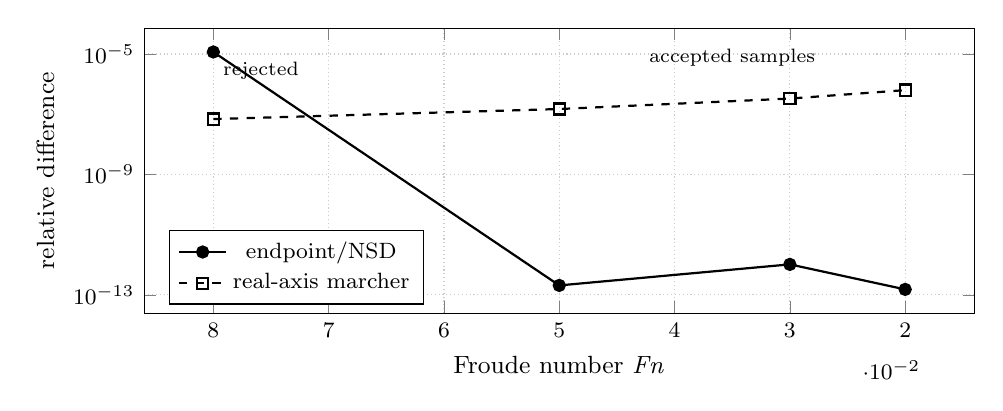
\begin{tikzpicture}
\begin{axis}[
  width=\linewidth,height=5.2cm,
  xlabel={Froude number $\Fn$},ylabel={relative difference},
  ymode=log,x dir=reverse,
  grid=major,major grid style={black!20,densely dotted},
  legend style={font=\footnotesize,draw=black,fill=white,
    at={(0.03,0.03)},anchor=south west},
  tick label style={font=\footnotesize},label style={font=\small}
]
\addplot+[black,solid,mark=*,mark options={fill=black},thick] coordinates {
  (0.08,1.172e-5) (0.05,2.070e-13) (0.03,1.034e-12) (0.02,1.526e-13)};
\addlegendentry{endpoint/NSD}
\addplot+[black,dashed,mark=square,mark options={solid},thick] coordinates {
  (0.08,6.918e-8) (0.05,1.493e-7) (0.03,3.322e-7) (0.02,6.334e-7)};
\addlegendentry{real-axis marcher}
\node[font=\scriptsize,text=black,anchor=north west]
  at (axis cs:0.08,1.172e-5) {rejected};
\node[font=\scriptsize,text=black,anchor=north]
  at (axis cs:0.035,3e-5) {accepted samples};
\end{axis}
\end{tikzpicture}
\end{minipage}\hfill
\begin{minipage}[t]{0.48\textwidth}
\centering
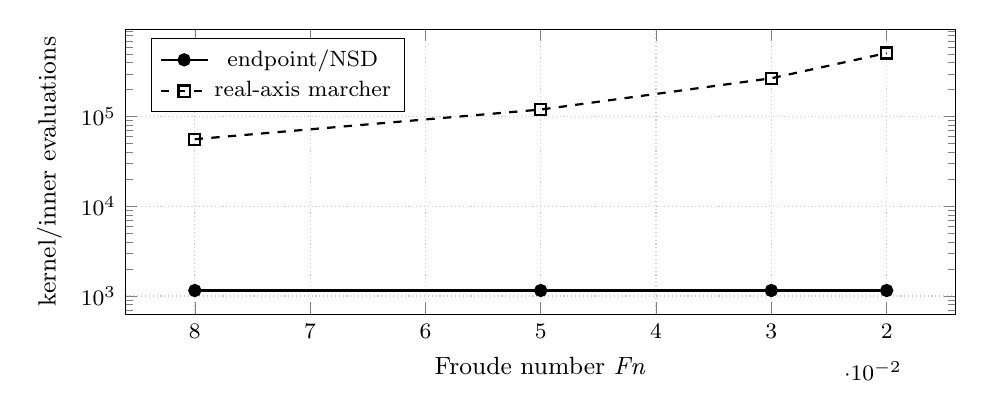
\begin{tikzpicture}
\begin{axis}[
  width=\linewidth,height=5.2cm,
  xlabel={Froude number $\Fn$},ylabel={kernel/inner evaluations},
  ymode=log,x dir=reverse,
  grid=major,major grid style={black!20,densely dotted},
  legend style={font=\footnotesize,draw=black,fill=white,
    at={(0.03,0.97)},anchor=north west},
  tick label style={font=\footnotesize},label style={font=\small}
]
\addplot+[black,solid,mark=*,mark options={fill=black},thick] coordinates {
  (0.08,1152) (0.05,1152) (0.03,1152) (0.02,1152)};
\addlegendentry{endpoint/NSD}
\addplot+[black,dashed,mark=square,mark options={solid},thick] coordinates {
  (0.08,56032) (0.05,119936) (0.03,267856) (0.02,511504)};
\addlegendentry{real-axis marcher}
\end{axis}
\end{tikzpicture}
\end{minipage}
\caption{Observed accuracy (left) and work (right) as Froude number decreases.
The independent reference resolves endpoint/NSD differences at the
\(10^{-13}\)--\(10^{-12}\) level, while geometry fixes its quadrature work.  At
default tolerance, the hybrid rejects the reduced result at
\(\Fn=0.08\) and accepts it at \(\Fn=0.05,0.03,0.02\).}
\label{fig:scaling}
\end{figure*}

\subsection{Runtime}

Timing used an optimized build, 30 samples per case, and the default relative
tolerance \(10^{-5}\).  Each case received its own unmeasured warm call.  The
two method comparisons alternated execution order on every sample; other cases
were sampled separately in the printed order.  Absolute timings are
host-dependent; the work counts and checksums are deterministic.  The host was
an Apple M5 MacBook Air running Darwin 25.5.0, with Rust/Cargo 1.96.0.

\begin{table*}[t]
\centering
\caption{Final release benchmark on the development host.}
\label{tab:timing}
\begin{tabular}{@{}lrrl@{}}
\toprule
Case & Median (ms) & IQR (ms) & Diagnostic\\
\midrule
21 speeds, \(\Fn=0.10\ldots0.50\) & 13.035 & 12.996--13.064 & corrected checksum\\
Default API, \(\Fn=0.05\) & 0.030 & 0.030--0.030 & 1,152 nodes\\
Real-axis marcher, \(\Fn=0.02\) & 21.506 & 21.464--21.557 & 511,504 evaluations\\
Endpoint/NSD, \(\Fn=0.02\) & 0.031 & 0.030--0.031 & 1,152 nodes\\
\bottomrule
\end{tabular}
\end{table*}

At \(\Fn=0.02\), the frozen paired run gives about a 700-fold median speedup.
Two immediately repeated paired runs gave 702--707-fold; an earlier cold-host
run gave 608-fold, while the former fixed-order reviewer protocol gave
approximately 750--865-fold.  We therefore do not treat any point ratio as
portable.  Cost changes little between \(\Fn=0.05\) and 0.02, as
\cref{eq:gaussian} predicts.  During the 21-speed design sweep, the hybrid
selects the path that satisfies the error gate.  The checksum is
\(2.553251156101\times10^5\); it differs from the pre-fix value because the
corrected marcher retains a positive tail that the earlier rule truncated.

\section{Analytic lineage and implementation scope}
\label{sec:prior}

The present solver revives a substantial analytic lineage.  The
equation-level comparison in \cref{tab:lineage} separates the historical
reductions from the implementation work reported here.  For the 1972 and 1988
papers, the table states only what their verified publisher or index records
establish; both full texts remain due-diligence items rather than dependencies
of our classification.

\begin{table*}[t]
\centering
\caption{Equation-level comparison of polynomial and basis reductions of
Michell resistance.  ``Record'' denotes a verified publisher or bibliographic
record where the full text was unavailable.}
\label{tab:lineage}
\scriptsize
\begin{tabular}{@{}p{0.15\textwidth}p{0.20\textwidth}p{0.20\textwidth}p{0.17\textwidth}p{0.17\textwidth}@{}}
\toprule
Source & Basis and reduction & Kernel or speed dependence & Error control and dispatch & Relation to this implementation\\
\midrule
Birkhoff--Kotik via \citet[eqs.~39--45]{Wehausen1973}
& Hull autocorrelation \(M(u,v)\), with equivalent \((P,Q)\) transforms and separable elementary ships
& Geometry-independent kernel \(K(\nu u,\nu v)\); a \(Y_0\) reduction is also reported
& Absolute convergence justifies the change of integration order
& Establishes separation of hull data from a reusable kernel\\
\addlinespace
\citet[eqs.~3.3--3.4]{Michelsen1960}
& Polynomial hull function \(H(\xi,\zeta)\) after the Birkhoff--Kotik transformation
& Michell function \(C(s,t)\) contains speed dependence
& Convergence conditions accompany the transformation
& Direct historical antecedent of shape/kernel separation\\
\addlinespace
\citet[eqs.~3.21--3.22, 3.38--3.40]{Michelsen1960}
& Monomial expansion of \(H\); each coefficient contributes through a closed series expression
& Confluent-hypergeometric, Bessel, and Struve functions; speed-and-degree terms can be tabulated
& Appendix proves series convergence; computer tabulation is proposed
& Antecedent of analytic polynomial reduction for design use\\
\addlinespace
\citet{Michelsen1972}, verified record
& Gegenbauer expansion of the centerplane Havelock-source distribution
& Orthogonality reduces resistance to a finite double sum depending on source coefficients, \(\Fn\), and length--draft ratio
& The accessible abstract states the reduction and identifies its governing inputs
& Published JSR continuation of the basis-reduction program\\
\addlinespace
\citet{SendagortaGrases1988}, verified record
& Products of integral shape functions
& Rapidly convergent series with linear, shape-independent velocity functions suitable for tabulation
& The abstract reports that few terms give suitable accuracy; detailed controls await source access
& Antecedent of separated, table-driven computer-aided design\\
\addlinespace
Present implementation
& Degree-\(\leq16\) tensor-product B-spline span polynomials reduced to active endpoint waves
& Continued Bickley pair kernels on a frequency-scaled Gaussian contour
& Coefficient, accumulation, omission, and quadrature estimates; explicit acceptance gate and real-axis fallback
& Modern error-accounted realization for coarse, well-separated endpoints\\
\bottomrule
\end{tabular}
\end{table*}

The implementation differs from that lineage in five engineering details:

\begin{enumerate}
  \item it operates span by span on tensor-product B-splines, including
        full-multiplicity chine knots;
  \item it restricts both spline degrees to the independently validated range
        1--16 and charges coefficient construction and endpoint cancellation;
  \item it bounds the resistance contribution of every omitted submerged
        endpoint pair;
  \item it evaluates retained \(K_s\) pairs on a frequency-scaled contour with
        a bounded, order-aware node count; and
  \item it accepts the reduction only when the combined estimate meets the
        requested tolerance, otherwise returning to the general marcher.
\end{enumerate}

These deltas are engineering improvements, not priority claims.  A full
method-by-method benchmark against the Michelsen and Sendagorta--Grases
representations lies outside this paper and remains future work.

The endpoint structure is also established independently.
\citet{KellerAhluwalia1976} express leading small-Froude resistance and waves
through bow and stern waterline slopes.  \citet{Gotman2002} repeatedly
differentiates polynomial hull functions, separates endpoint self terms from
bow--stern interference, and discusses higher endpoint derivatives.  Our
finite B-spline decomposition puts that mechanism into implementation form; it
does not introduce a new physical asymptotic principle.

Tuck and Lazauskas also establish exact or Filon-like integration of
piecewise-polynomial inner data \citep{Tuck1989,Lazauskas2009}.  As
\citet{Lazauskas2009} describes it, Michlet combines exact
piecewise-quadratic longitudinal formulas with a fixed angular rule.  Our
solver retains the same thin-ship physics but, for accepted B-spline hulls,
keeps low-Froude outer work from growing with frequency.  We classify that result
as an engineering improvement and make no head-to-head performance claim
against the Michlet executable.  Exact endpoint reduction also survives the
outer modulus square: pair expansion converts it into a small set of reusable
special-function kernels.  Ruffa and Toni give finite Bessel--Struve module
representations for integer-order Bickley functions \citep{RuffaToni2026};
their stability on the imaginary axis remains to be tested as a possible
kernel backend.

Contour deformation is well established for oscillatory quadrature
\citep{HuybrechsVandewalle2006}.  \citet{Motygin2017} applies steepest descent
and Clenshaw--Curtis quadrature in ship-wave theory, but to the oscillatory part
of the Kelvin Green function rather than Michell's resistance integral.
Automated methods now handle general phases and coalescing saddles
\citep{GibbsHewettHuybrechs2024}.  Such methods could treat multihull transverse
phases; the present quadratic phase needs only the closed contour in
\cref{eq:gaussian}.

\section{Limitations and open extensions}
\label{sec:limits}

The evidence covers a narrow model: upright symmetric monohulls in linear,
deep-water thin-ship theory.

\begin{itemize}
  \item \textbf{Geometry.}  The reduced solver supports upright symmetric
        single hulls of degree 1--16 in each spline direction.  Its active
        endpoints must satisfy \(\nu|x_i-x_j|\geq25\), so it targets coarse,
        well-separated endpoint maps.  Asymmetric, heeled, multihull, and
        closely spaced cases fall back to the general method.
  \item \textbf{Error certification.}  The submerged-pair omission bound and
        Gaussian tail bound are analytic.  The selected coarse/fine quadrature
        difference and floating-point roundoff are not interval-certified.
  \item \textbf{Reference floor.}  The independent real-axis reference uses
        compensated summation through \(\lambda=4000\); at \(\Fn=0.02\), a
        cutoff-doubling check changes it by \(1.23\times10^{-15}\).  Differences
        near the observed \(10^{-13}\) scale are resolution measurements, not
        interval-certified digits.
  \item \textbf{Physical model.}  Michell theory is linear, inviscid, slender,
        deep-water, and fixed-attitude.  At very low speed, viscous effects may
        dominate the already small wave resistance.  For free-surface flow
        past singular obstacles, low-Froude waves can be exponentially small,
        beyond all algebraic orders, and controlled by Stokes phenomena; that
        different problem is not resolved by better quadrature
        \citep{TrinhChapman2015}.
\end{itemize}

The highest-leverage numerical extension is multihull support.  A transverse
placement introduces phase
\(\nu y\lambda\sqrt{\lambda^2-1}\) and moving saddles that
\cref{eq:gaussian} does not contain.  A uniform or automated contour must
account for them.  Retaining shallow submerged endpoints likewise produces
mixed linear and quadratic complex phases.  Further work should certify the
contour error, test imaginary-argument Bickley recurrences, derive finite-depth
kernels, and differentiate the endpoint representation for low-Froude hull
optimization.

\section{Conclusions}

Finite integration by parts converts the B-spline inner transform into endpoint
waves.  Pair expansion then turns the outer modulus square into continued
Bickley kernels, and contour rotation replaces real-axis oscillation with
Gaussian decay.  Geometry, rather than Froude number, sets the reduced
quadrature work.  The submerged-pair bound lets the hybrid reject the reduction
whenever it exceeds the requested tolerance.

For the standard Wigley hull at \(\Fn=0.02\), the reduced solver is more
accurate than the general marcher and about 700 times faster in the frozen
paired run.  This
result is an engineering improvement for the supported geometry, built from
the analytic reduction lineage summarized in \cref{tab:lineage}.  Claims
beyond the current scope require broader geometry and certified total error
control.

\section*{Reproducibility statement}

The implementation, tests, benchmark harness, generated results, and number
audit are available in the public
\href{https://github.com/risingtideresearch/michell}{\texttt{michell}
repository}.  On acceptance for submission, the immutable source, test, and
artifact package will be archived and the placeholder
\href{https://doi.org/\ArchiveDOI}{\nolinkurl{\ArchiveDOI}} replaced with its
minted DOI.  The current numerical kernel will be identified by the immutable
local tag \texttt{paper-a-jsr-v2}; that tag will not be moved after creation.

\section*{Acknowledgments}

We conducted this work for the Rising Tide Research Foundation.  Under the
authors' direction, OpenAI Codex substantially drafted the manuscript and
assisted with code development, numerical experiments, and literature mapping.
The authors reviewed and edited the material, independently checked the cited
sources and numerical evidence, and accept full responsibility for the
content.

\bibliographystyle{plainnat}
\bibliography{references}

\end{document}
